	\documentclass[11pt]{article}

\usepackage{fullpage}
\usepackage[margin=1in]{geometry}
\usepackage{graphicx}
\usepackage{amsmath,amsthm,amssymb}
\usepackage{hyperref}
\usepackage{biblatex}
\usepackage[dvipsnames]{xcolor}



\addbibresource{references.bib}

\graphicspath{ {./} }

% --------------------------------------------------------------
%                         Start here
% --------------------------------------------------------------

\begin{document}

\title{C Group Project Final Report}
\author{Hoang Vu, Kaiyan Fan, Xuan(Tom) Zhao, Zelin(Daniel) Deng}

\maketitle

\noindent In this group project, we have accomplished ARM11-based emulator and assembler, as well as \texttt{Tetris++} for our extension. Below is our final report.

% --------------------------------------------------------------
%                         ARM11 Assembler
% --------------------------------------------------------------

\section{ARM11 Assembler}

% --------------------------------------------
%             Assembler Structure
% --------------------------------------------
\subsection{Assembler Structure}
\begin{figure}[!ht]
  \centering
  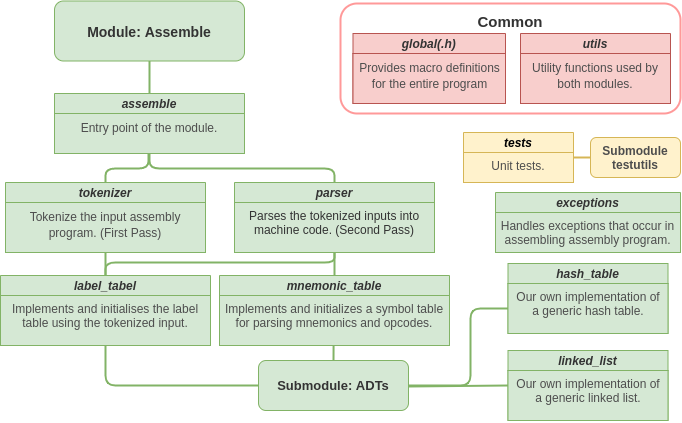
\includegraphics[scale = 0.55]{project_structure_assemble.png}
  \caption{An UML Diagram of the Assembler. The \texttt{testutils} and \texttt{adts} are in directory \texttt{\textbackslash lib}}
  \label{part1:UML}
\end{figure}
\begin{flushleft}
The functions of different parts are described in the diagram above. For the assembler, there are three main parts: symbol table, tokenizer, and parser. For the symbol table, we have implemented both \texttt{linked\_list} and \texttt{hash\_table}, and we finally chose \texttt{hash\_table} as the implementation for \texttt{symbol\_table}. In the first pass, when the assembler reads the assembly code, each line is tokenized into a \texttt{struct} containing label, opcode, and operand fields separately; then, in the second pass, this \texttt{struct} will be parsed into binary code by the \texttt{parser} with the help of \texttt{label\_table} and \texttt{mnemonic\_table}. We have previously intended to use the data structure we defined in \texttt{instructions.h} in the emulator as an intermediate structure, but that turns out to be over-complicate and unnecessary. 
\end{flushleft}

% --------------------------------------------
%             Implementation
% --------------------------------------------

\subsection{Implementation}
\begin{flushleft}
Here's some data types we have defined several in our assembler that are worth mentioning:
\begin{itemize}
\item \texttt{symbol\_table\_t} is the mapping between strings (such as mnemonics and labels) and binaries, implemented using a hash table. The \texttt{label\_table} and \texttt{mnemonic\_table} use this structure.
\item \texttt{assembly\_line} contains \texttt{label}, \texttt{opcode}, an array of \texttt{operands} strings for each operand fields, and a \texttt{location\_counter} for tracking the address of a label in instruction memory.
\item \texttt{mnemonic\_t} contains the 32-bit binary determined by the opcode and the instruction type.
\item \texttt{machine\_code} contains the binary code of an entire assembly file and the line count of binary code.
\end{itemize}
Before the first pass begins, the \texttt{mnemonic\_table} is initialized. The \texttt{mnemonic\_table} maps mnemonics into \texttt {mnemonic\_t} structures that contain 32-bits binary codes and instruction type. For the 32-bits binary codes, the bits that can not be determined solely from mnemonics (such as bits representing register address) will be left with 0. Then, in the first pass, the tokenizer performs lexical analysis to tokenize each line of assembly code into \texttt{assembly\_line} structure. Any labels encountered are inserted into the \texttt{label\_table} with their corresponding address. Next, in the second pass, the parser queries the \texttt{mnemonic\_table} to determine the instruction type and the 32-bits binary code (the bits that can be determined directly from the mnemonics are set correctly by the \texttt{mnemonic\_table}). Afterward, the \texttt{parser} breaks down different operand fields according to the instruction type and sets the rest of the bits according to the operands. For branching instructions, the addresses of the labels are determined by querying the \texttt{label\_table} and the offset can be therefore calculated. Finally, the binary instruction is appended to the \texttt{machine\_code}, which will be outputted by the \texttt{write\_binary\_file} function in \texttt{utils.c} after the second pass complete.
\end{flushleft}
\begin{flushleft}
Additionally, we have added the ability to handle possible exceptions and encapsulated as many structures as possible. For instance, we have written getters and setters in out table implementation. We also defined \texttt{eMalloc}, \texttt{eCalloc}, and \texttt{eRealloc} functions, which checks for \texttt{NULL} pointers before returning the pointer to the allocated memory.
\end{flushleft}


% --------------------------------------------------------------
%                         Extension: Tetris++
% --------------------------------------------------------------

\section{Extension: Tetris\texttt{++}}

\begin{figure}[!ht]
  \centering
  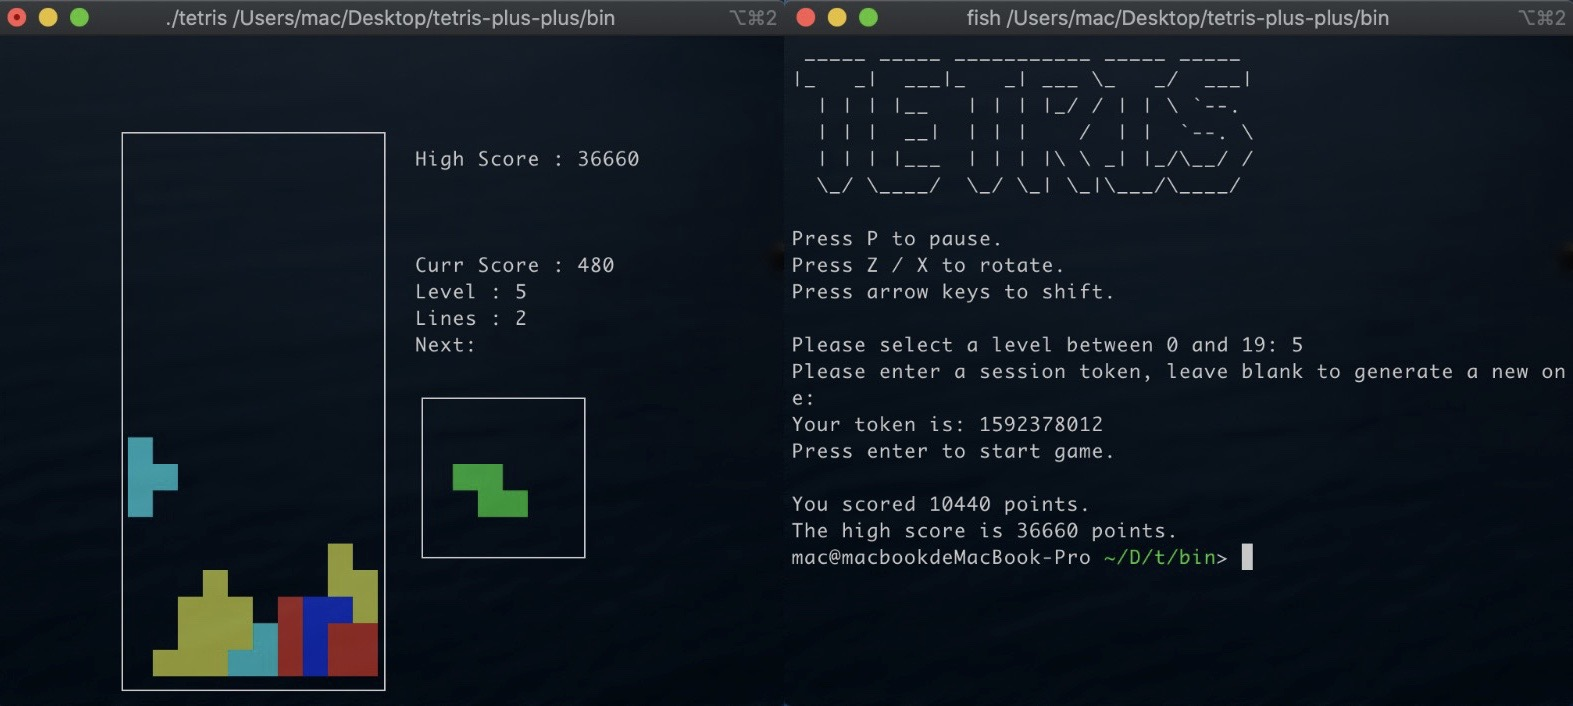
\includegraphics[scale = 0.25]{tetris.jpg}
    \caption{A Demo of the Tetris Interface in Command Line}
  \label{part2:jpg}
\end{figure}


% --------------------------------------------
%             Description
% --------------------------------------------

\subsection{Description}

\begin{flushleft}
Tetris is a game loved by all of our team members, and Tetris++ a way to stay healthy both mentally and physically during the quarantine by playing Tetris. We provide interactive ways to play tetris through Tetris Pi, and you can also compete with AI through Tetris Buddy. It is also a world-class Tetris player, able to match even the strongest human contenders.
\end{flushleft}

\begin{flushleft}
The first version of AI used genetic algorithm. We devised four optimization factors in playing Tetris: aggregate height across each column, the number of complete lines formed, number of holes, and bumpiness(the sum of total differences between adjacent columns). The AI will first generate random parameters to multiply with these factors, then it will calculate the best move based on this score. The fittest ones(those that can get more lines cleared) will be selected to form the next generation. Each generation has 100 children and this process will repeat for 1000 times.
\end{flushleft}

\begin{flushleft}
After this very successful bot, we have decided to tackle another big challenge employing Q-Learning technique in introducing a second bot to compute with the first. The main aim of this part is to compare to effectiveness of Genetic Algorithm and Q-Learning for this particular task.

\end{flushleft}

\begin{flushleft}
The raspberry PI mode provides three more interactive ways to play the game: button, sports, and rhythms (so no keyboard required anymore). The wiring setup is specified in the corresponding source files. "Button" mode is for playing Tetris with a controller that have five buttons. "Sports" mode is for playing Tetris by jumping up and down and stretching your arms and legs, using infrared motion sensors, ultrasonic distance sensors, and sound sensors. "Rhythms" mode is for playing Tetris with two controllers equipped with gyroscopes and accelerometers. They detect the motion of the controllers and the Tetris blocks can be controlled by moving or rotating the controller. There are also LED array displays, which displays an incomplete 8*16 (standard Tetris is 10*20) board. We originally planned for a "driving" mode, but due to malfunctioning sensors, it is not implemented. 
\end{flushleft}

% --------------------------------------------
%             How to play
% --------------------------------------------

\subsection{How to Play}

\begin{flushleft}
Please see the README in the repository for compilation instructions. After compilation, the executables would be located in the \texttt{bin} directory. To play in classic Tetris mode, run \texttt{./tetris}. The player has to pick a level to start with, then chooses to put in a random number as a seed. The higher the level, the faster the game. The control keys are shown on the welcome screen: press \texttt{P} to pause, press \texttt{Z / X} to rotate the block, press arrow keys to move left or right.
\end{flushleft}

\begin{flushleft}
If you want to play alongside the conservative AI, run \texttt{./genetic-ai-play conservative}; if you are feeling risky, run \texttt{./genetic-ai-play risky}. If you have a Raspberry Pi with the correct sensors, run ./tetrispi to play Tetris Sports and Tetris Rhythms. 
\end{flushleft}

% --------------------------------------------
%        Challenges and Problems
% --------------------------------------------

\subsection{Challenges and Problems}

\subsubsection{Game Engine}
\begin{flushleft}
The core algorithm of Tetris is relatively simple. To help with consistency and standardisation, we chose to use the reverse engineering of the 1989 NES Tetris as the standard for how the game should behave \cite{tetrisreverseengineering}. We chose this version as it is a popular implementation that all future versions evolved from. The challenge is to design a system of inputs and outputs that are versatile enough for all of our extensions, whilst being easy to use for the users. For example, games employ a system called DAS (delayed auto-shift), to make sure both "taps" and "holds" of a key are being registered correctly, and getting the timing right for this part was challenging. In the end, we decided to sample the input at the rate of 60 times per second, which allowed seamless user input without the use of multi-threading. 
\end{flushleft}

\subsubsection{Raspberry Pi}
\begin{flushleft}
The raspberry PI version for \texttt{Tetris++} uses many sensors to detect input, and uses two \texttt{LED arrays} to display the board. The major challenge is to allow Raspberry Pi to communicate with these chips. They use different protocols (such as \textit{i2c} and \textit{spi}), and the \texttt{LED arrays} we used don't even have documentation, so it took a while to figure out how to communicate with them correctly. Another issue is with the control flow. Although 60FPS frame rate is fine for console input, the sensors and the \texttt{LED arrays} can't function properly without being constantly refreshed. This forces us to create separate threads to execute infinite loops for refreshing the LED arrays and some sensors. We even encountered race conditions when we were developing. The most annoying part of hardware-related development is with debugging. It is difficult to distinguish between bugs with the code, errors with wiring, and malfunctioning sensors, so we have to go through additional steps to determine the source of bugs. We have once spent 2 hours looking for a bug on the \texttt{LED array} display, and only found out that we connected the power PIN to 3.3V, instead of the 5V PIN required.
\end{flushleft}

\subsubsection{Tetris AI}
Here, we have taken this opportunity to experiment with two famous algorithms, Genetic Algorithm which is mainly used in optimisation problems, and Reinforcement Learning, specifically using the Q-Learning Model. The biggest common challenge for both AI implementations is the evaluation of a \textit{good} move. The instinct tells us that a good move should fit the shape of the bottom layer which will make the line as flat as possible, but it is hard to quantify this. After spending a few hours on research, we have decided to use a modified policy taken from \cite{tetrisai} including \textit{aggregate height, number of lines cleared, number of holes and bumpiness}, as illustrated.  

\paragraph{Tetris AI - Genetic Algorithm}
\begin{flushleft}
The challenge of the genetic AI is not its implementation, but its design and also to represent a good move. One issue is how to design a good way to reduce calculations and changes to arrays to save time during training. For instance, our implementation has separated the current generation and its children into two arrays instead of merging them. We have also encapsulated the clone functions for the state and the grid, though partial clone might be faster. It turns out that the training progress is comparatively fast if running on a multi-core server.
\end{flushleft}


\paragraph{Tetris AI - Reinforcement Learning}
\begin{flushleft}
The fundamental idea is to reward the bot when it performs a beneficial move and comparing that against its experience. To do this, we need to give our agent a memory, or more precisely the state of the game along with the outcome of each action. On first sight, the Tetris Board can be represented as a binary matrix, where 0 for a blank and 1 for an occupied cell. However, this can easily add up to ${2^{300}}$ possible states, including the states of our block. Hashing was our first solution, which quickly shows its weakness as not only it was challenging coming up with a hash function that captures the state of the block and the board. Our second attempt was to encode the Tetris Board using an array of heights, relative to the height of the first column. From our research, this is usually solved by employing other AI techniques, mainly Deep Learning to find a good mapping for dimensionality reduction. However, due to time constraints of implementing such a network, and a further constraint of training time, we leave this as a future improvement.
\end{flushleft}

    
% --------------------------------------------
%             Testing
% --------------------------------------------

\subsection{Testing}
\begin{flushleft}
We have implemented test cases for each module in our extension the same way we had done in emulator and assembler. We have unit tests for every function that can be tested in the core module. To improve the effectiveness of our testing, members are discouraged to write their tests for their module. Instead, we have the responsibility of writing tests for each other, using only the descriptions in the specification as a way of reducing bias. Integration tests in this module are done by trying edge cases in the input fields, and by spending time manually running the program. More than 20 hours of test time has been spent on the core module alone. 
\end{flushleft}

\begin{flushleft}
For the genetic algorithm, the test cases only cover some functions. To validate whether the training is on the right track, we run it on a server for a while to see if the number of lines cleared is increasing after training each generation.
\end{flushleft}

\begin{flushleft}
There's no way to test the hardware without actually running it. We played the game on raspberry Pi many times to ensure no significant bugs can be found. However, constrained by the accuracy of the hardware itself, occasionally the inputs are not detected correctly.
\end{flushleft}

% --------------------------------------------------------------
%                         Reflection
% --------------------------------------------------------------

\section{Reflection}

% --------------------------------------------
%             Group reflection
% --------------------------------------------

\subsection{Group reflection}
\begin{flushleft}
Our group holds a high standard during our development. With our frequent use of git, we have communicated efficiently, divided work by using git issues and reviewed each other's codes using merge requests. We used git issues to create a separate branch for every new development, which is merged into development when it passes our unit tests; development is then merged into master when it passes all the provided test cases. Each group member has also contributed in writing test cases for different modules. This workflow helps us avoid bad merge conflicts or potential bugs. 
\end{flushleft}

\begin{flushleft}
Because of our clear communication and agile workflow, the difference in timezone worked in our favour as it allowed a near 24-hour development cycle with enough overlap for code review sessions. 
\end{flushleft}

\begin{flushleft}
There remains a potential for improvements as well, especially for researches and plannings. For example, we changed the structure of the assembler halfway, which is a waste of time and efforts. If we have done more researches about two-pass assembling before designing the assembler, we could save a lot of time. We should also manage our time better, such as deciding on what to do for the extension earlier so we have more time for improvements. We also should try to code together on a shared working space using plug-ins like "live share" next time. Although Git is a great tool, coding together helps the whole group to gather more ideas and achieve better code quality. This is also a great way to avoid merge conflicts when we attempt to modify the same file together.
\end{flushleft}

% --------------------------------------------
%             Individual Reflection
% --------------------------------------------

\subsection{Individual Reflection}
\begin{itemize}
    \item Hoang Vu: I truly see the power of teamwork after this group project. As a team, we have clearly shown the effectiveness of group discussions and the importance of feedback. As individuals, we have all shown a high level of dedication to our work, as well as review each other's work. Having our strengths, our ideas were very creative and diverse, which ultimately led to the success of this project.  Personally, my biggest lesson was being able to write reusable codes which I got from writing our \texttt{ADT hash\_table}. This was then used in \texttt{mnemonic\_table, label\_table} and \texttt{q\_table}. One possible improvement is that we should be discussing ideas on how to approach problems together before coding it up, this will reduce the amount of time that we waste from completely re-designing a particular functionality after negative feedback.    
    \item Kaiyan Fan: I spent much of my time structuring the project and reviewing my teammates' code. This is the first time I tried to review other people's code, and it turns out to be a very beneficial process. By reviewing code, I learnt what kind of code is difficult to read for code reviewers, and I hope I'll, therefore, write more readable code in the future. I also learnt many git commands from my teammates. One thing I should improve is to think about my teammates' suggestions and ideas more carefully. Sometimes I just stick to my own opinion and didn't think about my teammates' suggestions thoroughly, but later I found out that my teammates are correct. I should listen to my teammates more carefully to save my own, and everyone's efforts and time. But overall, I believe I have cooperated with this team successfully and efficiently. I have made good contributions and learnt a lot from my teammates.
    \item Xuan(Tom) Zhao: During this group project, I have developed the decoder in emulator and part of the parser in assembler. I wrote the AI with a genetic algorithm in our extension and trained different version of it. At first, I thought communication is my limiting factor, but it turns out that both the code reviews and our zoom meetings are rather productive. The real limiting factor that I need to tackle is to add more care when writing code. The most important lesson I have learned from this group work is that design is the most pivotal step, and good design could reduce code size and complexity, and eventually fewer bugs to deal with.
    \item Zelin(Daniel) Deng: Whilst Kaiyan did a brilliant job structuring the C dependencies, I was in charge of the physical layout. On top of writing my share of the C code, I structured the repositories and Makefiles for versatility and modularity. I learnt first hand the power of teamwork as sometimes one problem you can't solve in a day can be solved by your teammates instantly through a different perspective. The rest of the group did a great job complimenting my strength in keeping files organised, and weaknesses in writing unit tests. I hope I complimented theirs as well. For future group work, I would spend more time helping to write tests for my teammates, in addition to testing my code.  
\end{itemize}


\printbibliography

\end{document} 